\begin{figure}[ht]
    \centering
    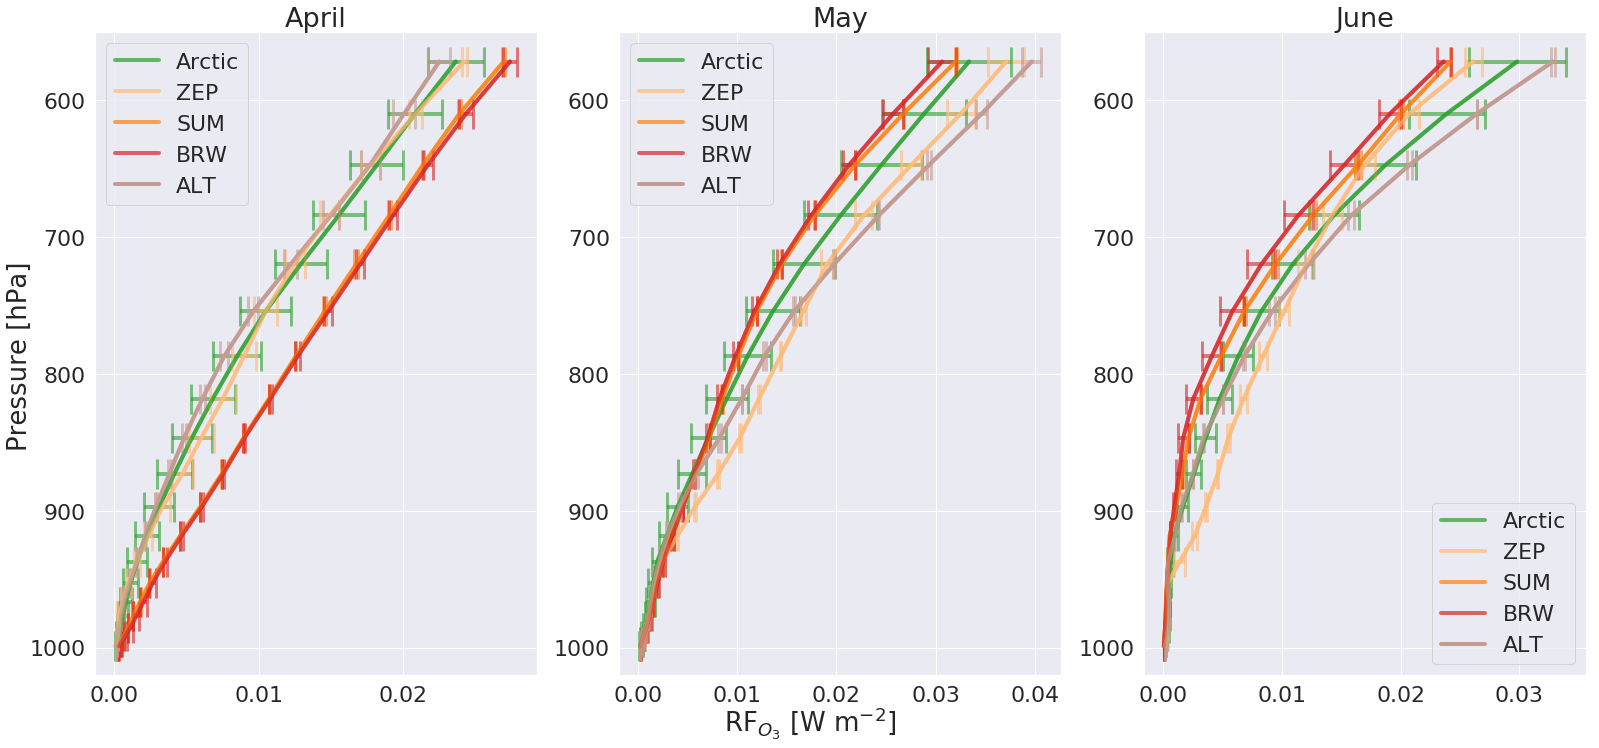
\includegraphics[width = \linewidth]{Chapter6_Results/images/RF/vert_RF_AprJune_2001.png}
    \caption{Monthly mean averaged RF (in Wm$^{-2}$) in each model layer (layer 1-60) averaged over the whole Arctic (defined as above 68$^o$N) (green line), over Zeppelin (77.0-80.5$^o$N, 10.5-13.5$^o$E) (yellow line), over Summit (71.0-74.0$^o$N, 40.0-37.0$^o$W)(orange line), over Barrow (70.0-73.0$^o$N, 40.0-37.0$^o$W)(red line) and over Alert (80.5-84.5$^o$N, 64.0-61.0$^o$W)(purple line). Errorbars indicate the standard deviation in the layer. The profiles are shown for the months April (left), May (middle) and June (right) in 2001}
    \label{fig:vert_RF_AprJune_2001}
\end{figure}


% diff_mean_SUM = find_stats_lev(diff, 'mean', 'O3_RF', 71.0, 74.0, 180-40.0, 180-37.0)
% diff_std_SUM = find_stats_lev(diff, 'std', 'O3_RF', 71.0, 74.0, 180-40.0, 180-37.0)
% diff_mean_ALT = find_stats_lev(diff, 'mean', 'O3_RF', 80.5, 84.5, 180-64.0, 180-61.0)
% diff_std_ALT = find_stats_lev(diff, 'std', 'O3_RF', 80.5, 84.5, 180-64.0, 180-61.0)
% diff_mean_BRW = find_stats_lev(diff, 'mean', 'O3_RF', 70.0, 73.0, 180-40.0, 180-37.0)
% diff_std_BRW = find_stats_lev(diff, 'std', 'O3_RF', 70.0, 73.0, 180-40.0, 180-37.0)
% diff_mean_ZEP = find_stats_lev(diff, 'mean', 'O3_RF', 77.0, 80.5, 180+10.5, 180+13.5)
% diff_std_ZEP = find_stats_lev(diff, 'std', 'O3_RF', 77.0, 80.5, 180+10.5, 180+13.5)